%Introduction
%\begin{savequote}[50mm]
%If our brains were simple enough for us to understand them, we'd be so simple that we couldn't.
%\qauthor{Ian Stewart }%The Collapse of Chaos: Discovering Simplicity in a Complex World
%\end{savequote}
%[Technologies for interoperable multi-device services]
\chapter{Fields of application}
\chaptermark{Fields of application}
\label{chap:fields}

\section{Overview}
The deployment presented in Chapter \ref{chap:deployment} and the generalisation of the adaptation methodology and the model presented in Chapter \ref{chap:adaptation} can be applicable to other fields different from the audiovisual and broadcasting. This means that the same methodology will provide a variation of the model that could be adapted for each case. More in detail, this chapter provides examples of two fields in which the applicability of the solution has been identified, based on a real technological demand from relevant stakeholders, where the technology has been adapted and transferred to them. In particular, the technology has been used by a company working in the industry and manufacturing sector, and by some relevant actors in the field of crisis environments. Next sections describe how media technologies can improve the actual way of operation in both cases, including the challenges to overcome and the research work and deployments completed so far. 

\section{Industry}
Recent developments in information and communication technology (ICT) and the latest Internet-related technologies are opening up revolutionary possibilities for manufacturing and production. The technology surrounding Industry 4.0 and smart factories is mainly focused in certain fields, such as the Internet of Things (IoT), industrial big data, industrial automation, cybersecurity or intelligent robotics. Nevertheless, it is important to emphasise the relevance of computer graphics and media technologies, under the
umbrella of visual computing as key enabling technologies in smart factories of the future.

\subsection{Media technologies and multi-screen media services for operators in Industry 4.0}
This section focuses on the role of the operator in the smart factory, which plays a crucial role within the vertical integration dimension in Industry 4.0. Smart factories change the role of operators, making new types of interaction possible between them and the machines. Therefore, human-centricity becomes a key concept, fostering the cooperation of machines and humans toward a more efficient and effective human-automation symbiosis. This concept is related to the Operator 4.0 term mentioned in \cite{romero2016operator}.

In this context, it is interesting to note that many authors explicitly identify augmented reality (AR) as one of the main Industry 4.0 technologies to empower the operator \cite{funk2016motioneap}. However, being that AR an important aspect with its own challenges and possibilities, we believe that a broader combination of computer graphics, vision and media technologies can be very important to support operators and to learn from their actions in new smart factory scenarios. In addition, support from knowledge-based and intelligent systems is critical in this context. We will present a set of challenges related to the operator in the context of smart factories along with current examples of relevant related R\&D activities in this field. 

Figure \ref{fig:industrycha} is an updated version of the figure in \cite{posada2018graphics} and shows the role of operators in smart factories, where three major challenges can be identified:
\begin{figure}
	\begin{center}
		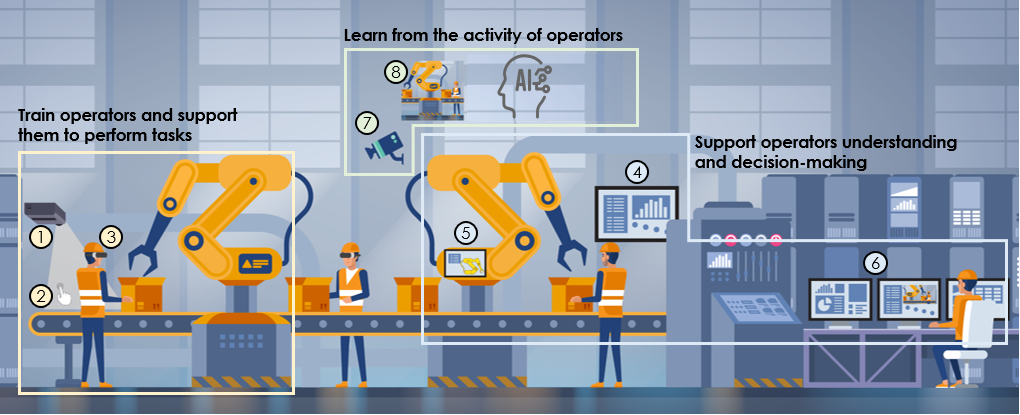
\includegraphics[width=1\textwidth]{industrychallenges.png}
		\caption{Challenges of the operators in Smart Factories}
		\label{fig:industrycha}
	\end{center}
\end{figure}

\begin{enumerate}
\item The first challenge is to support operators performing tasks within a process or workflow. In this context, AR plays a crucial role with improved experiences, projecting instructions with the next steps of the workflow onto objects and tools (Figure~\ref{fig:industrycha}, number~1), or enabling projection-based gestural interaction (Figure~\ref{fig:industrycha}, number~2). Moreover, AR technologies and devices can overcome limitations of operators with disabilities or special needs (Figure~\ref{fig:industrycha}, number~3). Virtual reality Reality (VR) is also a relevant enabling technology for training activities.

\item The second challenge is to support operators’ understanding and decision-making in all the activities throughout the production process to provide an adequate ecosystem to optimally perform tasks. More versatile and enhanced human-machine interfaces (HMI) are needed, following a human-centred approach and facilitating analytical reasoning through interactive multi-screen interfaces with visual analytics. They need to address operators using different screens, such as shared big screens (Figure \ref{fig:industrycha}, number 4), and specific machine HMIs (Figure \ref{fig:industrycha}, number 5) or personal devices (such as smartphones or tablets). All these screens must provide a consistent overview of data and information in the form of graphs or media presentations (Figure \ref{fig:industrycha}, number 6), personalising the visualisation for each operator’s role, and enabling ubiquity to address operators’ movement from one set of screens to another.

\item The third challenge is to learn from the operators’ activities to predict specific situations, optimise the process and better organise the smart factory. In this context, video management capabilities (recording, streaming, etc.) are fully required with a complete integration of the Manufacturing Execution System(MES) (Figure~\ref{fig:industrycha}, number 7). On the one hand, video management will enable real-time supervision of the tasks both from inside or outside the premises, while providing an enriched reporting of the production process. On the other hand, artificial intelligence techniques such as pattern recognition and machine (deep) learning make it possible to learn from operators’ tasks and influence in the process (Figure \ref{fig:industrycha}, number 8). 

\end{enumerate}

From the three mentioned challenges the second one is closely related with the work presented in Chapter \ref{chap:deployment} and Chapter \ref{chap:adaptation} and it leads us to think about how Dynamic multi-screen dashboards for operators in Industry 4.0 would be.

\subsection{Dynamic multi-screen dashboards for operators in Industry 4.0}
Traditional industrial HMIs are very “static,” mostly based on old (WIMP \footnote{Windows, Icons, Menus and Pointers}) interaction paradigms. More specifically, industrial HMI interaction includes basically some alarms, basic production output data and production planning, and some sensor information. Most of the information offered to operators and engineers is based on static text, pictures in the best cases, and specially data (diagrams, statistics, etc.), shown in external screens attached to the machines, in PC stations close to production, or on normal displays in the shop floor. Production dashboards are a very clear case for this. In order to have better knowledge of the real production environment, a very powerful tool, not sufficiently used in state of the art industrial practice, is needed to capture and use the relevant events in video. It is noteworthy that there is very little adoption of video recording, management, search, etc. in real-world factories.

A recent trend is to include mobile devices for dashboards and other functionalities to some extent, but the approach is based on expensive rugged hardware that runs proprietary software
solutions with single-screen paradigms, highly rigid and fixed distribution of information in the screen, and few interaction possibilities.


\begin{figure}
	\begin{center}
		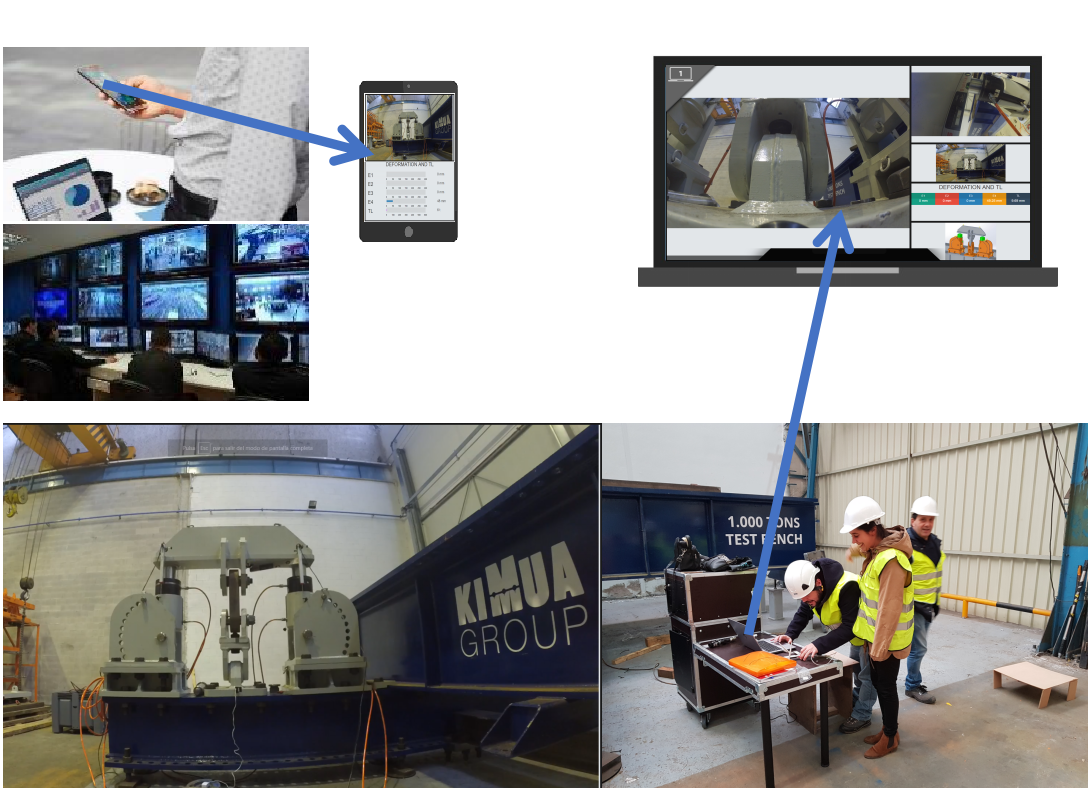
\includegraphics[width=1\textwidth]{industrypilot.png}
		\caption{Example of a pilot done in the industry field}
		\label{fig:indpilot}
	\end{center}
\end{figure}

\begin{figure}
	\begin{center}
		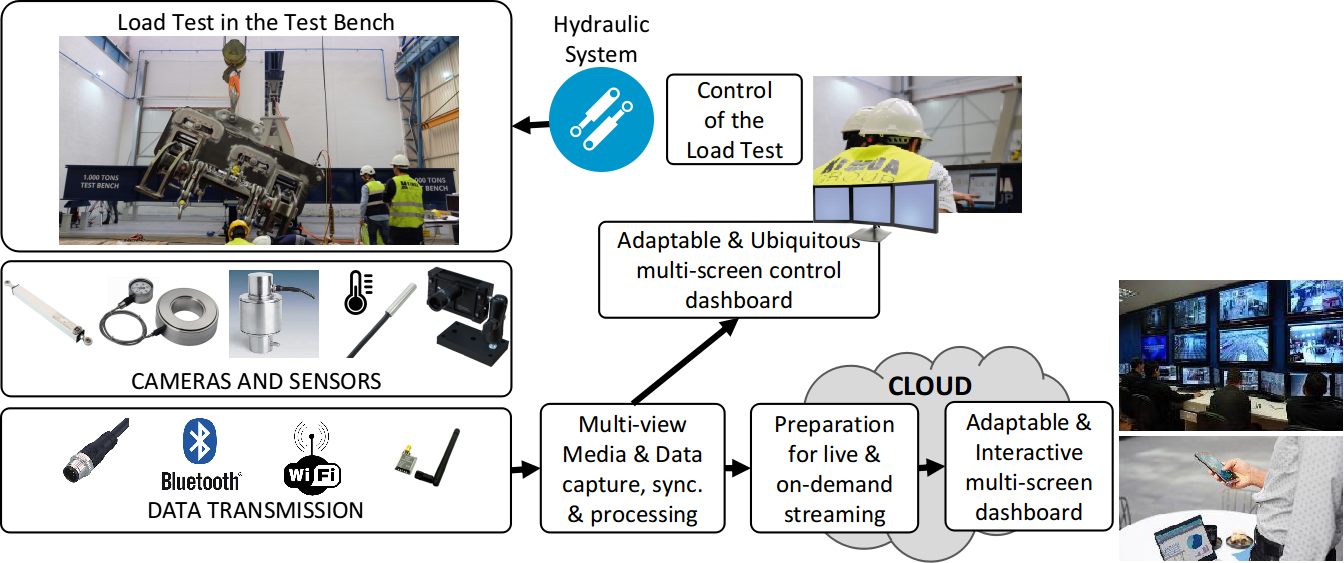
\includegraphics[width=1\textwidth]{industrydash.png}
		\caption{Dynamic multiscreen dashboards for operators in Industry 4.0}
		\label{fig:industrydash}
	\end{center}
\end{figure}

Our current research example involves the development of a core dashboard system for an industrial, export-oriented SME that builds tools for heavy lift operations and that owns a modular,
portable and monitored Test Bench to perform Load Tests. This is a typical industrial case: An engineer controlling the load test through a specific hydraulic system, with its own HMI, while the outcome information of the test is displayed through different interfaces in machine-specific displays. A team of distributed operators is visually controlling the load test and following the different displays, interacting with the engineer to fine-tune the test. As the tests are run in international locations, the engineer has to physically travel to the sites.
This is a case of horizontal integration of Industry 4.0, in which emerging Internet-based systems allow a deeper integration between industrial clients and providers, empowering operators and engineers to work collaboratively even in remote international locations, and avoiding the need of costly physical travel and ad-hoc adaptations of user interfaces. Figure \ref{fig:indpilot} and Figure \ref{fig:industrydash} show the pilot tested in this field. In this context, a more versatile and smart solution was desired, providing:
\begin{itemize}
	\item An ubiquitous, adaptable and very flexible multi-screen dashboard to monitor multiple camera views and the outcome data in real time, in order to have all the information when controlling the load test through the hydraulic system.
	\item A live adaptable and flexible multi-screen visualisation solution for engineers around the world to follow the load test remotely, as they were on the premises, combining graphics and media with all the relevant information in an interactive and customisable multi-device interface,
	\item An on-demand inspection solution of the load test, personalising the view and verifying all the process and the adequate performance of the test, and the generation of an added value advanced and interactive report as a communication tool for engineers to learn more about the tools that are being measured. 
\end{itemize}


This provides an adaptable and ubiquitous multi-screen control dashboard, where different video sources and heterogeneous outcome data are captured and prepared to be exposed through a
Web-based HTML-5 application. All information is shown in any kind of Web-based device, such as a laptop, a tablet or a smartphone. The pieces of information and user interface layout is dynamically configured according to the target device and enables the interaction of the operator. Different devices can be easily associated, such as multiple laptops and mobiles being used by the same operator, and the user interface dynamically adapts to that multi-screen configuration, showing parts of the application on each screen, and enabling the operator to move components from one device to another. Moreover, the operator can move from one place to another in the premises, dissociating big screens and having all the relevant information in the mobile, while associating new big screens in the new location.
Current deployment is well accepted by operators and engineers as it opens more efficient ways to get information and communicate the tests.

In a dashboard like the one described in this section, a multi-screen user interface adaptation model such as the one presented in Chapter \ref{chap:adaptation} could be very valuable since it could automatically distribute the components among the connected devices, providing a responsive layout in each of them. Furthermore, if the model was enriched through a continuous learning processes, the system would know which configuration is the best for each scenario.   



\section{Crisis environments}

Technology can also contribute greatly to crisis environments, especially by enhancing the interconnectedness between the authorities and the public services and by facilitating the rapid exchange of heterogeneous information. Crises take on a variety of shapes and forms —natural or health disasters, terroristic and criminal acts, technology malfunctions, and large-scale accidents— at local, regional, national, and global levels. Crisis management plans, created and implemented at the organisational level, typically involve public services and institutional authorities overseeing emergency response. 

In this context, media technologies can facilitate cooperation within
response organisations or the response network, but also can enable wider cooperation such as citizen collaboration. To achieve these ends, crisis practitioners and crisis managing operators are calling for multi-screen technologies that allow to manage multiple sources of information that take into account the perceptions, needs, and practices of multiple users. 

\subsection{Media technologies and multi-screen media services for crisis environments}

This section focuses on media technologies that ease a more efficient crisis management, making the exchange of multiple sources of information possible between authorities and public services. 

In this context, it is interesting to note that solutions that allow the distribution of multiple video signals in any environment by means of low delay adaptive streaming protocols are important to empower the crisis management. Moreover, we believe that, again, broader combination of computer graphics, vision and other media technologies can be very important to extend the information provided by the video signals and offer to the target viewer the sources that are relevant to make the corresponding decisions. That way, media, text or image components could be helpful to better understand what is happening in each moment and allow to manage and organise all the involved stakeholders, each one with its specific action area. In addition, support from knowledge-based and intelligent systems are also essential in this field. 

Figure \ref{fig:crisischa} shows the main challenges to manage a crisis environment backed by media technologies.

\begin{figure}
	\begin{center}
		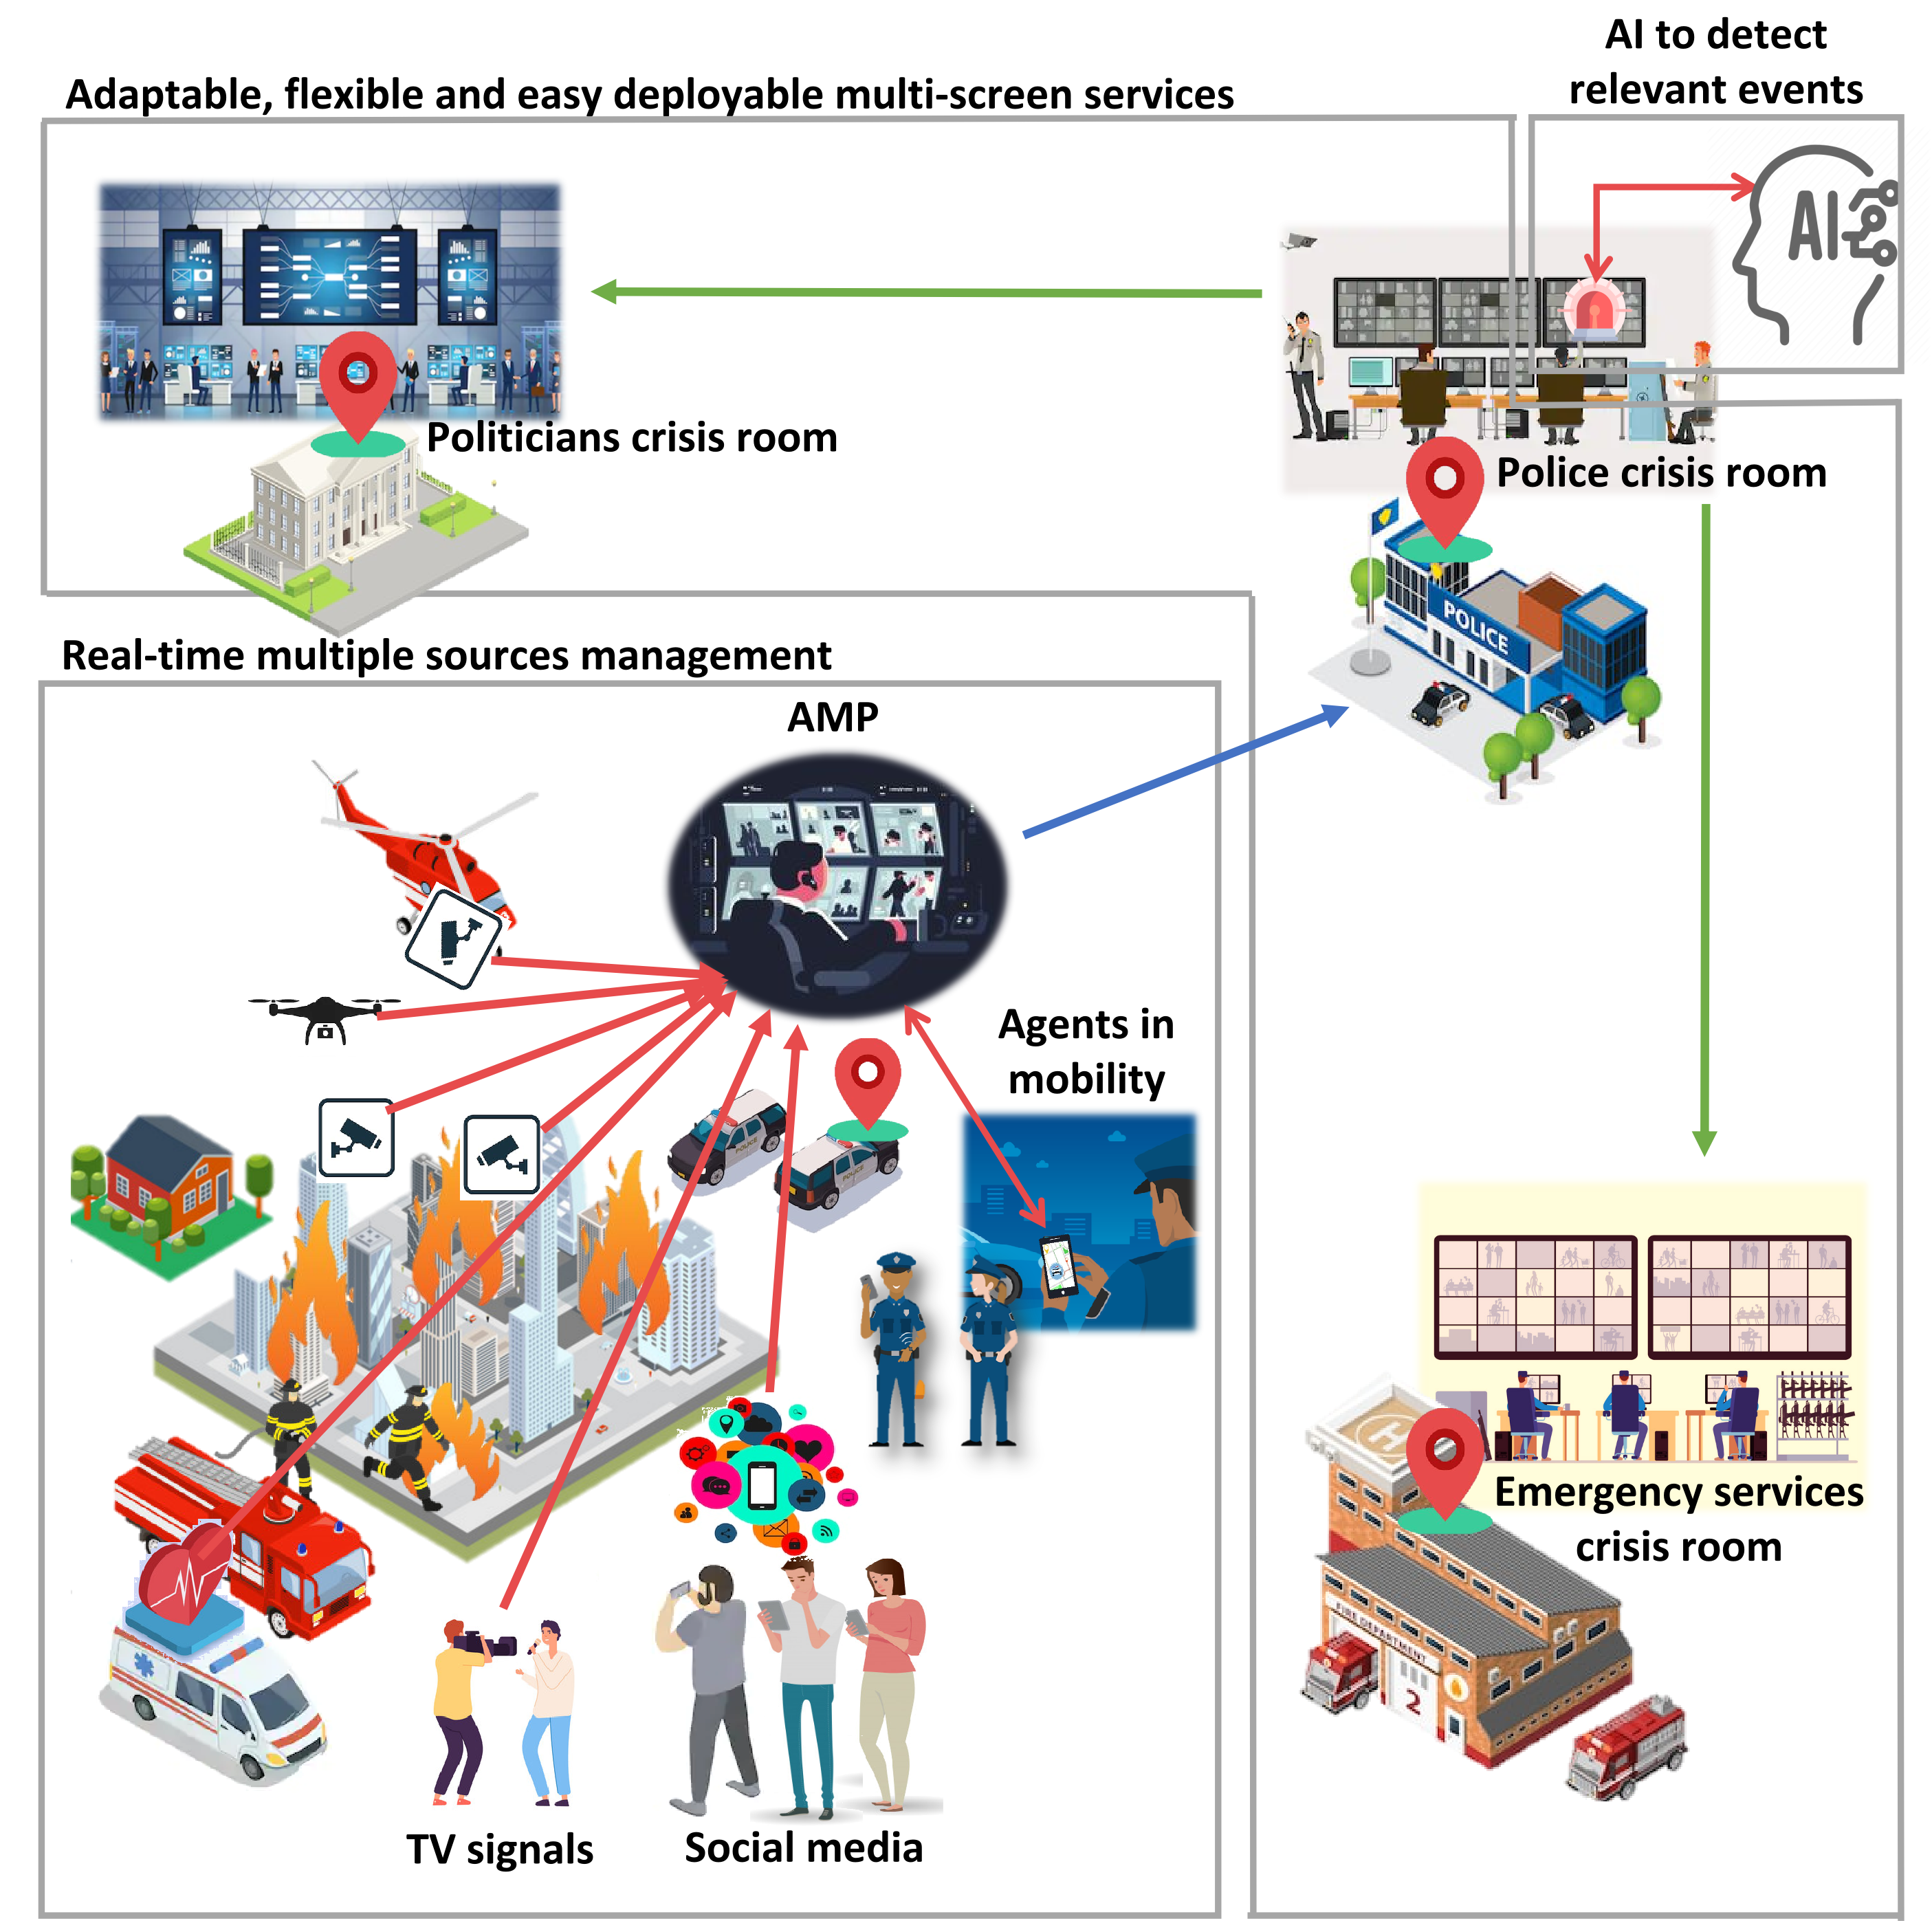
\includegraphics[width=1\textwidth]{crisischallenges.png}
		\caption{Example of a crisis environment}
		\label{fig:crisischa}
	\end{center}
\end{figure}

\begin{enumerate}
\item The first challenge is to cope with multiple video and data signals coming from any environment. This includes, security cameras installed in buildings, TV signals, drones, agents in mobility, data monitored by sensors, social media or even any valuable data found on the Internet. In this context video management capabilities are fully required to enable real-time monitoring of the crisis. 

\item The second challenge is to provide an adaptable, flexible and easy deployment multi-screen media service that allows to centralise and manage several information sources not only based on video signals but also on data extracted from the Internet and authorities' internal data systems. And all of these avoiding to use proprietary softwares and expensive hardware depending solutions. These solutions need to address operators using different screens, such as video-walls, laptops or personal devices. All of these screens, which are used to be able to perform a forensic analysis and look over the occurrences, must provide a consistent overview of data and information taking into account the role of the target visualiser. 

\item The third challenge is to learn from operators interaction to make even faster the deployment of the needed resources and be able to manage the crisis efficiently from the beginning. Additionally, artificial intelligence techniques over video signals such as object detection and tracking or face recognition could be very helpful to create alarms when a relevant event is identified. 
\end{enumerate}

From the mentioned challenges the second one is closely related with the work presented in Chapter \ref{chap:deployment} and Chapter \ref{chap:adaptation} and it leads us to think about how Dynamic multi-screen dashboards for crisis environments would be. 

\subsection{Dynamic multi-screen dashboards for crisis environments}

Nowadays different data and video system approaches are used depending on the requirements of each scenario. Therefore, solutions are based on video-walls depending on expensive hardware that runs proprietary software solutions, with highly rigid and fixed distribution of information in the screens, and few interaction possibilities.

In this context we see another interesting opportunity to migrate recent technology advances from other areas with intensive interaction based on dynamic, mobile, multiple screens toward crisis monitoring scenarios, which remove the hardware and proprietary software dependencies and provide a wider range of communication and information sharing possibilities. 


\begin{figure}
	\begin{center}
		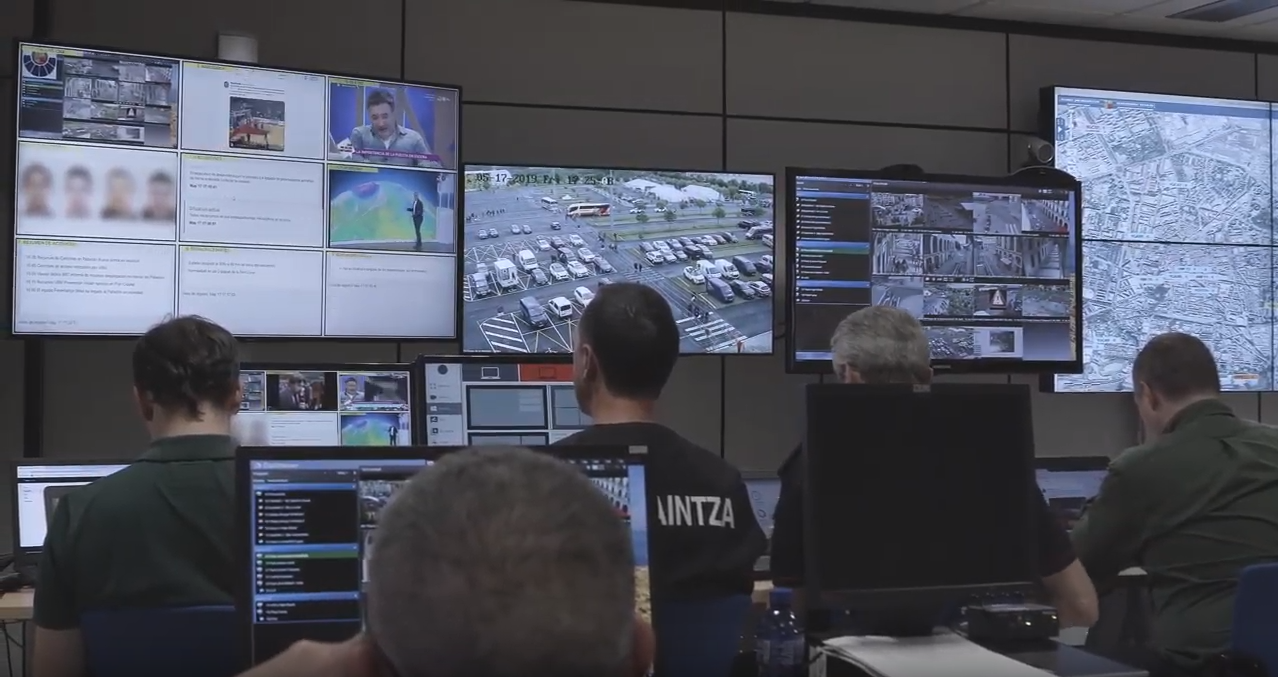
\includegraphics[width=1\textwidth]{crisispilot.png}
		\caption{Example of a pilot done in a crisis environment}
		\label{fig:cripilot}
	\end{center}
\end{figure}

A current research example involves the development of a pilot that allowed to monitor an sport event such as the Final Four of the Basketball Euroleague that took place in Vitoria-Gasteiz. In this pilot, several information sources were managed by an administrator that had direct view of each source and decided which components to see in each connected screen both in situ and remotely. Furthermore, he was able to decide the layout template to represent the information in each case.
In addition, a team of content managers was be able to operate all the range of content sources, including several video flows, TV signals, investigation information, reserved data, performed action register, public cooperation information, suspects' images, social network entries or even any valuable information found on the Internet. Figure \ref{fig:cripilot} shows the pilot tested in this environment. 

A similar approach was also implemented to monitor a football match of the Spanish league that took place in San Mamés stadium in Bilbao, with the goal of testing a pilot that allows to monitor some matches of the UEFA Euro 2020 that will take place in the same stadium. 

Again, these solutions provide an adaptable and ubiquitous multi-screen control dashboard, where different many heterogeneous sources are centralised and prepared to be exposed through a
Web-based HTML-5 application. All the information can be shown in any kind of Web-based device, such as a laptop, a tablet or a smartphone. Information can be easily controlled, operated and shared through multiple screens being used by one or multiple users simultaneously and the user interface dynamically adapts to that multi-screen configuration, showing parts of the application on each screen, and enabling the crisis managing operator to move components from one device to another and share the information in accordance with the role of each agent. Moreover, the system allows agents in mobility receiving or providing relevant information by means of the mobile phone. Current deployment is being well accepted by authorities and engineers as it opens more efficient ways to get information and communicate the tests.

Once again, in a solution like the one described in this section, a multi-screen user interface adaptation model such as the one presented in Chapter \ref{chap:adaptation} could be very valuable since it could automatically distribute the components among the connected devices, providing a responsive layout to each of them. Furthermore, if the model was enriched through a continuous learning processes, the system would know which configuration is the best for each scenario.  


\section{Common approach}

Once the previous fields have been analysed, it is interesting to see how to migrate recent technology advances from other areas with intensive interaction based on dynamic, mobile, multiple screens towards smart factory and crisis scenarios. Table \ref{tab:comparison} shows that the broadcast field that apparently is far away from industry and crisis contexts, is quite close in terms of user needs and specifications: we refer to the research advances in the dynamic adaptation of multiple screen visualisation and interaction for professional TV experiences, and its synergies with other media (Internet, etc.). 

\begin{table}
	\centering
	\caption{Analysis of the needs of TV viewers in broadcasting, industry 4.0 operators in smart factories and crisis managing operators in terms of dynamic multiscreen visualisation and interaction, emphasising the common aspects}
	\label{tab:comparison}
	\begin{tabular}{||m{4.5cm}|m{4.5cm}|m{4.5cm}||}
		\hline
		\textbf{TV spectator needs} & \textbf{Industry 4.0 operator and engineers needs} & \textbf{Crisis managing operator needs} \\
		\hline
		Ubiquitous media experience in TV screen, mobile devices, tablets, PCs. & Ubiquitous production information in multi-screen format & Ubiquitous multi-source information in multi-screen format (videowalls, mobile devices, etc.)\\
		\hline
		Harmonisation of TV broadcast signal with various Internet based information sources & Harmonisation of heterogeneous data sources (production plan, sensors, CAD, ERP, MES...) & Harmonisation of heterogeneous data sources (security cameras, tv signals, agents in mobility, sensor data, social media, news, etc. )\\
		\hline
		Dynamic synchronisation of social network inputs, Internet updates, multiple cameras input. & Dynamic synchronisation of sensor data, product design and production planing, even video streams to be able to perform a forensic analysis and look over the processes. & Dynamic synchronisation of video streams, sensor data, action planning or social media to be able to perform a forensic analysis and look over the ocurrences. \\
		\hline
		Personalised experience, relevant to user tastes and interests, interaction preferences, devices.& Personalised experience, relevant to the particular operator profile and task requirements. & Personalised experience, relevant to the particular crisis managing operator, authorities and emergency services according to their role and expertise. \\
		\hline
		Automatic localized information according to environment (e.g. in a car, in TV proximity, in a mobile) & Automatic localized information according to specific machine, location in plant.& Automatic localized information according to specific problem location. \\
		\hline
	\end{tabular}
\end{table}


More generally, the common features required by all the cases to succeed (including the broadcast field) would be: 
\begin{itemize}	
	 \item Web-based, HTML-5 and Web3D compliant technologies to obtain a fully interoperable service. 
	 
	 \item Multi-source content management to integrate heterogeneous data into the experience. Data fusion and the interoperability is based on standards.
	 	 
	 \item Detection and identification of available screens or devices to distribute the content making the most of the resources. 
	 
	 \item Information flow between screens to obtain a seamless experience.
	
	 \item Dynamic time-based alignment and synchronisation of data sources to obtain a coherent visualisation of the content across all the connected screens.
	
	 \item Dynamic adaptation model, to be able to distribute the content across the available screens and produce responsive and interactive visualisation based on user profile. 
\end{itemize}
	 
All the aforementioned proves that there are environments with the necessity of this kind of solutions and in which the methodology presented in Chapter \ref{chap:adaptation} is applicable. An effort would be required to characterise the components, devices and layouts in each case in order to generate an specific model in each situation, but the methodology would avoid the definition of an extensive set of rules.  
